\documentclass[tikz,border=4pt]{standalone}
% Shared art direction for the "phones" post, after Vagrancy's region art
% (vagrancy/analysis/art/regions.py and data/palette.json "art"): flat fills,
% plum ink lines, a mustard sky, peach and sage. Every colour below is copied
% from that palette so the post and the game look like one hand drew them.
%
% The scenes share a horizon at y=2.6 and the same sky band, so consecutive
% figures read as one continuous walk down the page.
\usetikzlibrary{arrows.meta,calc,decorations.pathmorphing}
\definecolor{ink}{HTML}{3B2A3F}
\definecolor{sky}{HTML}{E9C46A}
\definecolor{skylight}{HTML}{F2DC98}
\definecolor{cloud}{HTML}{F6E7B8}
\definecolor{peach}{HTML}{EBA77C}
\definecolor{peachdark}{HTML}{D98B5C}
\definecolor{cream}{HTML}{F3E6C4}
\definecolor{sage}{HTML}{9DB58A}
\definecolor{sagedark}{HTML}{6F8F66}
\definecolor{olive}{HTML}{B9B566}
\definecolor{teal}{HTML}{79ADA4}
\definecolor{tealdark}{HTML}{4F8580}
\definecolor{slate}{HTML}{6E8494}
\definecolor{stone}{HTML}{C9B79C}
\definecolor{wood}{HTML}{A9774E}
\definecolor{gold}{HTML}{E3B04B}
\definecolor{shadow}{HTML}{5B4A63}
\tikzset{
  ln/.style={draw=ink, line width=0.9pt, line join=round},
  thinln/.style={draw=ink, line width=0.6pt, line join=round},
  lab/.style={font=\sffamily\scriptsize, text=ink, align=center},
  tag/.style={font=\sffamily\scriptsize\bfseries, text=ink, align=center},
}
% A walking figure. #1 x, #2 y, #3 body colour, #4 head tilt in degrees
% (0 upright, negative looking down at a phone).
\newcommand{\walker}[4]{%
  \begin{scope}[shift={(#1,#2)}]
    \filldraw[fill=#3, ln] (-0.13,0) rectangle (0.13,0.52);
    \draw[ln] (-0.09,0) -- (-0.14,-0.28);
    \draw[ln] (0.09,0) -- (0.17,-0.26);
    \begin{scope}[rotate around={#4:(0,0.52)}]
      \filldraw[fill=cream, ln] (0,0.66) circle (0.14);
    \end{scope}
  \end{scope}}

\begin{document}
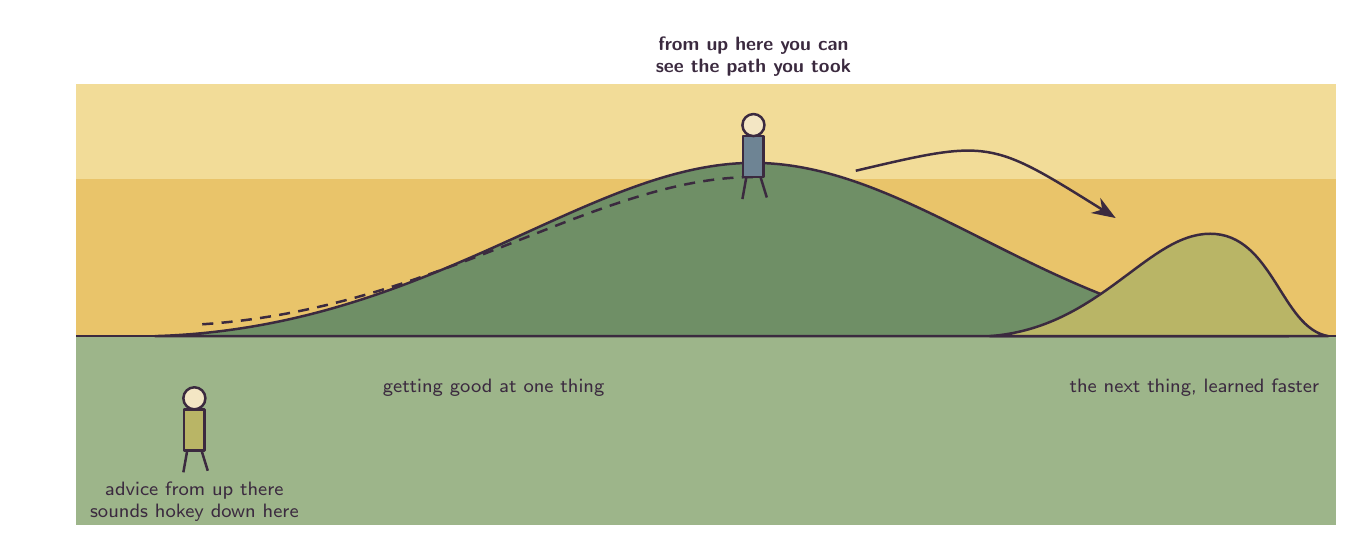
\begin{tikzpicture}[font=\sffamily]
  \fill[sky] (0,2.4) rectangle (16,5.6);
  \fill[skylight] (0,4.4) rectangle (16,5.6);
  \fill[sage] (0,0) rectangle (16,2.4);
  \draw[ln] (0,2.4) -- (16,2.4);
  % One hill, climbed. The vantage point is the whole argument: you can only
  % look back at a path you have already walked.
  \filldraw[fill=sagedark, ln] (1.0,2.4) .. controls (4.5,2.5) and (6.5,4.6) .. (8.6,4.6)
      .. controls (10.7,4.6) and (12.5,2.5) .. (15.4,2.4) -- cycle;
  \draw[ln, dash pattern=on 4pt off 3pt] (1.6,2.55) .. controls (4.6,2.75) and (6.6,4.42) .. (8.6,4.42);
  \node[lab, text width=4.4cm] at (5.3,1.75) {getting good at one thing};
  \walker{8.6}{4.42}{slate}{0}
  \node[tag, text width=4.6cm] at (8.6,5.95) {from up here you can see the path you took};
  % The second hill, not yet climbed, reached faster because of the first.
  \draw[ln, -{Stealth[length=3mm]}] (9.9,4.5) .. controls (11.6,4.9) .. (13.2,3.9);
  \filldraw[fill=olive, ln] (11.6,2.4) .. controls (13.0,2.5) and (13.6,3.7) .. (14.4,3.7)
      .. controls (15.2,3.7) and (15.3,2.5) .. (15.9,2.4) -- cycle;
  \node[lab, text width=3.2cm] at (14.2,1.75) {the next thing, learned faster};
  % The child who has not climbed anything.
  \walker{1.5}{0.95}{olive}{0}
  \node[lab, text width=4.0cm] at (1.5,0.3) {advice from up there sounds hokey down here};
\end{tikzpicture}
\end{document}
